\documentclass[a4paper]{report}
\usepackage{graphicx}


\title{Vaja 32 Sklopljeno nihalo}
\graphicspath{{./images/} }
\author {Jure Kos}
\date {5.1.2022}

\begin{document}
\maketitle

\chapter*{Uvod}

Nihalo, ki je sestavljeno iz dveh enakih težnih nihal in povezano z vzmetjo, se imenuje sklopljeno nihalo. 
Brez vzmeti, nihali nihata neodvisna drug od drugega, z vzmetjo pa
nihali postaneta odvisna drug od drugega. Nihanje sklopljenega nihala lahko opišemo z dvema lastnima nihanjema.\\
Prvo lastno nihanje je nihanje nihal, ki sta bili pognani v isti smeri z enakima sunkoma. Nihali nihata kot, da sta neodvisna drug od drugega in vzmet ne vpliva na nihanje.
Frekvenca, ki je enaka neodvisnima nihaloma, se imenuje prva lastna frekvenca.\\
Drugo lastno nihanje je nihanje nihal, ki sta bili pognani v nasprotnih smereh z enakima sunkoma. Nihali nihata z enako amplitudo in vzmet se krči in razteguje. Zaradi tega
nastane navor, ki je odvisen od koeficienta vzmeti in prijemališča vzmeti. Nihali nihata hitreje. Nihanje se imenuje drugo lastno nihanje, frekvenca pa druga lastna frekvenca. \\
Če eno nihalo odklonimo za določeno amplitudo, medtem ko je drugo v ravnovesni legi, in prvega spustimo, nihali začneta utripato. Do tega pride, ker se energija iz nihajočega nihala
prenese na nenihajoče nihalo in vlogi se zamenjata. Nihali nihata z nihajnim časom $t'$ in frekvenco $\omega'$. Čas $T$ je čas med dvema mirovanjima istega nihala in iz časa T dobimo
frekvenco utripanje $\omega_{u}$.

\chapter*{Naloga}

Opazuj sklopljeno nihanje dveh enakih fizičnih nihal! Izmeri in izračunaj lastni krožni frekvenci $\omega_0$ in $\omega_1$ ter še $\omega'$ in $\omega_u$! Določi koeficient vzmeti, izračunaj D' in faktor sklopitve $K = D' / (D + D')$!

\begingroup

\let\clearpage\relax

\chapter*{Potrebščine}

\begin{itemize}
\item Nihali na stojalu;
\item vzmeti za sklopitev;
\item merilo za določevanje koeficienta vzmeti;
\item centimetrsko merilo, kljunasto merilo;
\item tehtnica
\item uteži 10g, 20g, 50g, 100g, 200g
\item štoparica
\end{itemize}

\endgroup

\begingroup

\let\clearpage\relax

\chapter*{Navodila}

\begin{enumerate}
\item Za vsako nihalo izmeri nihajni čas za 30 nihajev ter izračunaj nihajni čas in frekvenco.
\item \begin{itemize}
  \item Nihali spni z vzmetjo.
  \item Odkloni nihali v isti smeri za enaki amplitudi in ju hkrati spusti. Izmeri čas 35 nihajev in izračunaj nihajni čas $t_0$ in lastno frekvenco $\omega_o$. Napravi 5 meritev.
  \item Odkloni nihali v nasprotnih smereh in izračunaj $t_1$ in $\omega_1$
  \item Eno nihalo zadrži v ravnovesni legi, drugo pa odmakni za amplitudo A ter obe nihali spusti hkrati. Izmeri čas 15 nihajev posameznega nihala in meritve za obe nihali ponovi
    dvakrat. Izračunaj nihajni čas  $t'$ in lastno frekvenco $\omega'$. Opazuj 3 mirovanja posameznega nihala in izračunaj čas $T$ in frekvenco utripanja $\omega_u$
  \end{itemize}
  \item Izmeri nihali in izračunaj vztrajnostni moment nihala $J$ in koeficient navora $D = mgd_0 $, kjer je $m$ masa nihala in $d_0$ razdalja od težišča do osi. Izračunaj volumen uteži in s pomočjo gostote medenine in aluminija
  izračunaj maso. Na vzmet obesi uteži z znano težo in izmeri raztezek. Določi koeficient $k$ iz grafa, kjer je na abcisni osi raztezek, na ordinatni osi pa sila. Izmeri še razdaljo
  $d$ od prijemališča vzmeti in osi nihala in izračunaj:  

\[
    D' = kd^2
\]
  
  Izračunaj $t_0$, $t_1$, $t'$ in $T$ in jih primerjaj z izmerjenimi. Vrednosti vnesi v tabelo.
\item Izračunaj faktor sklopitve z izmerjenimi $\omega_0$ in $\omega_1$, nato pa še z izračunanima $D$ in $D'$ in primerjaj rezultata.
    \[K = \frac{D'}{D+D'} = \frac{1-(\frac{\omega_0}{\omega_1})^2}{1 + (\frac{\omega_0}{\omega_1})^2}\]
\end{enumerate}

\endgroup

\chapter*{Nihajni čas in frekvenca neodvisnih nihal}

Izmerjen čas 30 nihajev $t_{30}$ delimo s številom nihajev $N$ in rezultat je nihajni čas $t_{0}$ enega nihaja. Lastno frekvenco $\omega_0$ se izračuna po formuli $\omega_0= \frac{2\pi}{t_0}$
\section*{Levo nihalo}

Izmerjen čas $t_{30L} = 55,32s \pm 0,01s$ \\
Nihajni čas $t_{0L}$:

\[
  t_{0L} = \frac{t_{30L}}{N} = 1,8s (1 \pm 0,0002)
\]

\noindent Lastna frekvenca $\omega_{0L}$:

\[
  \omega_{0L} = \frac{2\pi}{t_0} = 3,4s^{-1} (1 \pm 0,0002)
\]
  
\section*{Desno nihalo}

Izmerjen čas $t_{30D} = 55,49s \pm 0,01s$ \\
Nihajni čas $t_{0D}$:

\[
  t_{0L} = \frac{t_{30D}}{N} = 1,8 (1 \pm 0,0002)
\]

\noindent Lastna frekvenca $\omega_{0D}$:

\[
  \omega_{0D} = \frac{2\pi}{t_0} = 3,4s^{-1} (1 \pm 0,0002)
\]

\chapter*{Prvo lastno nihanje}

Meritve časa 35 nihajev sklopljenih nihal z odmikom v isto smer z enako amplitudo:

\begin{center}
  \begin{tabular}{| c | c |}
    \hline
    Poskus & $t_{35}$ \\ \hline
    1 & 64,81s \\ \hline
    2 & 64,81s \\ \hline
    3 & 64,58s \\ \hline
    4 & 64,78s \\ \hline
    5 & 64,84s \\
    \hline
  \end{tabular}
\end{center}

\noindent Povprečen čas $\overline t = 64,76s$ \\
Odstopanje $\Delta t = 0,18s$\\
Relativna napaka $\delta_{t0} = 0,003$ \\
Nihajni čas  $t_0$:
\[
  t_0= 1,8s (1 \pm 0,003)
\]
Lastna frekvenca $\omega_0$:
\[
  \omega_0 = 3,4s^{-1} (1 \pm  0,003)
\]

\chapter*{Drugo lastno nihanje}

Meritve časa 35 nihajev sklopljenih nihal z odmikom v nasprotno smer z enako amplitudo:

\begin{center}
  \begin{tabular}{| c | c |}
    \hline
    Poskus & $t_{35}$ \\ \hline
    1 & 59,34s \\ \hline
    2 & 59,86s \\ \hline
    3 & 59,37s \\ \hline
    4 & 59,35s \\ \hline
    5 & 58,84s \\
    \hline
  \end{tabular}
\end{center}

\noindent Povprečen čas $\overline t = 59,35s$ \\
Odstopanje $\Delta t = 0,51s$\\
Relativna napaka $\delta_{t1} = 0,009$ \\
Nihajni čas  $t_1$:
\[
  t_1= 1,7s (1 \pm 0,009)
\]
Lastna frekvenca $\omega_1$:
\[
  \omega_1 = 3,7s^{-1} (1 \pm  0,009)
\]

\chapter*{Utripanje}

Meritve časa 15 nihajev posameznega nihala, kjer je eno odmakneno iz ravnovesne lege za določeno amplitudo, in drugo nihalo, ki ostane v ravnovesni legi. Čas T je čas med dvema utripoma
nihala, $\omega_u$ pa frekvenca tega utripanja.

\section*{Desno nihalo}

\begin{center}
  \begin{tabular}{| c | c |}
    \hline
    Poskus & $t_{15}$ \\ \hline
    1 & 27,40s \\ \hline
    2 & 27,35s \\ \hline
    3 & 27,61s \\
    \hline
  \end{tabular}
\end{center}

\noindent Povprečen čas $\overline t = 27,45s$ \\
Odstopanje $\Delta t = 0,16s$ \\
Relativna napaka $\delta_{t'_D} = 0,006$ \\
Nihajni čas $t'_D$:

\[
  t'_D = 1,8s (1 \pm 0,006)
\]

\noindent Lastna frekvenca $\omega'_D$:

\[
  \omega'_D = 3,9s^{-1} (1 \pm 0,006)
\]


\section*{Levo nihalo}

\begin{center}
  \begin{tabular}{| c | c |}
    \hline
    Poskus & $t_{15}$ \\ \hline
    1 & 27,84s \\ \hline
    2 & 27,43s \\ \hline
    3 & 28,54s \\
    \hline
  \end{tabular}
\end{center}

\noindent Povprečen čas $\overline t = 27,91s$ \\
Odstopanje $\Delta t = 0,6s$ \\
Relativna napaka $\delta_{t'_L} = 0,02$ \\
Nihajni čas $t'_L$:

\[
  t'_L = 1,8s (1 \pm 0,02)
\]
\noindent Lastna frekvenca $\omega'_L$:

\[
  \omega'_L = 3,4s^{-1} (1 \pm 0,02)
\]

\section*{Povprečje levega in desnega nihala}

Čas $t' = 1,9s(1 \pm 0.01)$ \\
Lastna frekvenca $\omega' = 3,4 (1 \pm 0,01)$
  
    
\section*{Utripi - izmerjeni podatki}

 Desno nihalo:

\begin{center}
  \begin{tabular}{| c | c |}
    \hline
    Poskus & Čas $T$ \\ \hline
    1 & 16,03s \\ \hline
    2 & 16,61s \\ \hline
    3 & 16,21s \\
    \hline
  \end{tabular}
\end{center}

\noindent Levo nihalo

\begin{center}
  \begin{tabular}{| c | c |}
    \hline
    Poskus & Čas $T$ \\ \hline
    1 & 16,89s \\ \hline
    2 & 16,58s \\ \hline
    3 & 17,52s \\
    \hline
  \end{tabular}
\end{center}

Povprečen čas $ \overline T = 16,64s$ \\
Odstopanje $\Delta t = 0,88s$ \\
Relativna napaka $\delta t = 0,05s $ \\
Čas med dvema utripoma $T = 16,6s (1 \pm 0,05)$ \\
Frekvenca utripanja $\omega_u = 0,4s^{-1}(1 \pm 0,05)$ \\
 
\section*{Utripi - izračunani podatki}

Čas $T$ se izračuna po enačbi:

\[
  \frac{1}{T} = \frac{1}{t_1} - \frac{1}{t_0}  ;  T = 20,4s (1 \pm 0,1)
\]

Lastno frekvenco $\omega_u$ se izračuna po enačbi:

\[
  \omega_u = \omega_1 - \omega_0 =  0,3s^{-1}(1 \pm 0,007)
\]

\noindent Izračunani podatki so višji od izmerjenih. Do tega je prišlo, ker je težko točno določiti, kdaj nihalo točno preneha nihati in kdaj ponovno začne. 


\chapter*{Računski del}

\section* {D in J}

Izračunaj $D = mgd_0$, kjer je $m$ masa nihala in $d_0$ dolžina od težišča do osi.
$d_0 = 97,5 cm \pm 0,1 cm$

\subsection*{Masa}

\subsubsection*{Aluminij}

Dolžina $l_{Al} = 97,5 cm \pm 0,1 cm $ \\
Polmer $r_{Al} = 0,5 cm \pm 0,1 cm $\\
Gostota $\rho_{Al} = 2700 \frac{kg}{m^3}$ \\
\noindent  (vir: http://www2.arnes.si/~oskratl1s/fizika/vsebine\%208\%20razred/\\
gostota/Tabela\%20gostot.htm)

\[
  m = \rho V = \rho Ol = \rho \pi r^2 l = 0,2 kg (1 \pm 0,4)
\]

\subsubsection*{Medenina}

Dolžina $l_{M} = 8,8 cm \pm 0,1 cm $ \\
Polmer $r_{Al} = 2,2 cm \pm 0,1 cm $\\
Gostota $\rho_{Al} = 8600 \frac{kg}{m^3}$ \\

\noindent  (vir: http://www2.arnes.si/~oskratl1s/fizika/vsebine\%208\%20razred/\\
gostota/Tabela\%20gostot.htm)


\[m = \rho V = \rho Ol = \rho \pi r^2 l = 1, 1 kg (1 \pm 0,1)\]

\noindent Skupna masa $m = 1,27 kg (1 \pm 0,1)$

\[
  D = mgd_0 = 1,27kg * 9,81 \frac{m}{s^2} * 0,87 m = 10,8 Nm (1 \pm 0,1)
\]

\[
  J = \frac{D}{\omega_0^2} =0,9 \frac{Nm}{s} (1 \pm 0,1)
\]


\section*{D' in k}

Tabela sile uteži in raztezka:

\begin{center}
  \begin{tabular}{| c | c |}
    \hline
    Sila [N] & raztezek [cm] \\ \hline
    $9,81 N * 10^{-2}$ & $0,5$ \\ \hline
    $19,6 N * 10^{-2}$ & $1$ \\ \hline
    $49,1 N * 10^{-2}$ & $2,7$ \\ \hline
    $78,5 N * 10^{-2}$ & $3,3$ \\ \hline
    $147 N * 10^{-2}$ & $5,6$ \\ \hline
    $196 N * 10^{-2}$ & $8,8$ \\
    \hline
  \end{tabular}
\end{center}

Graf:

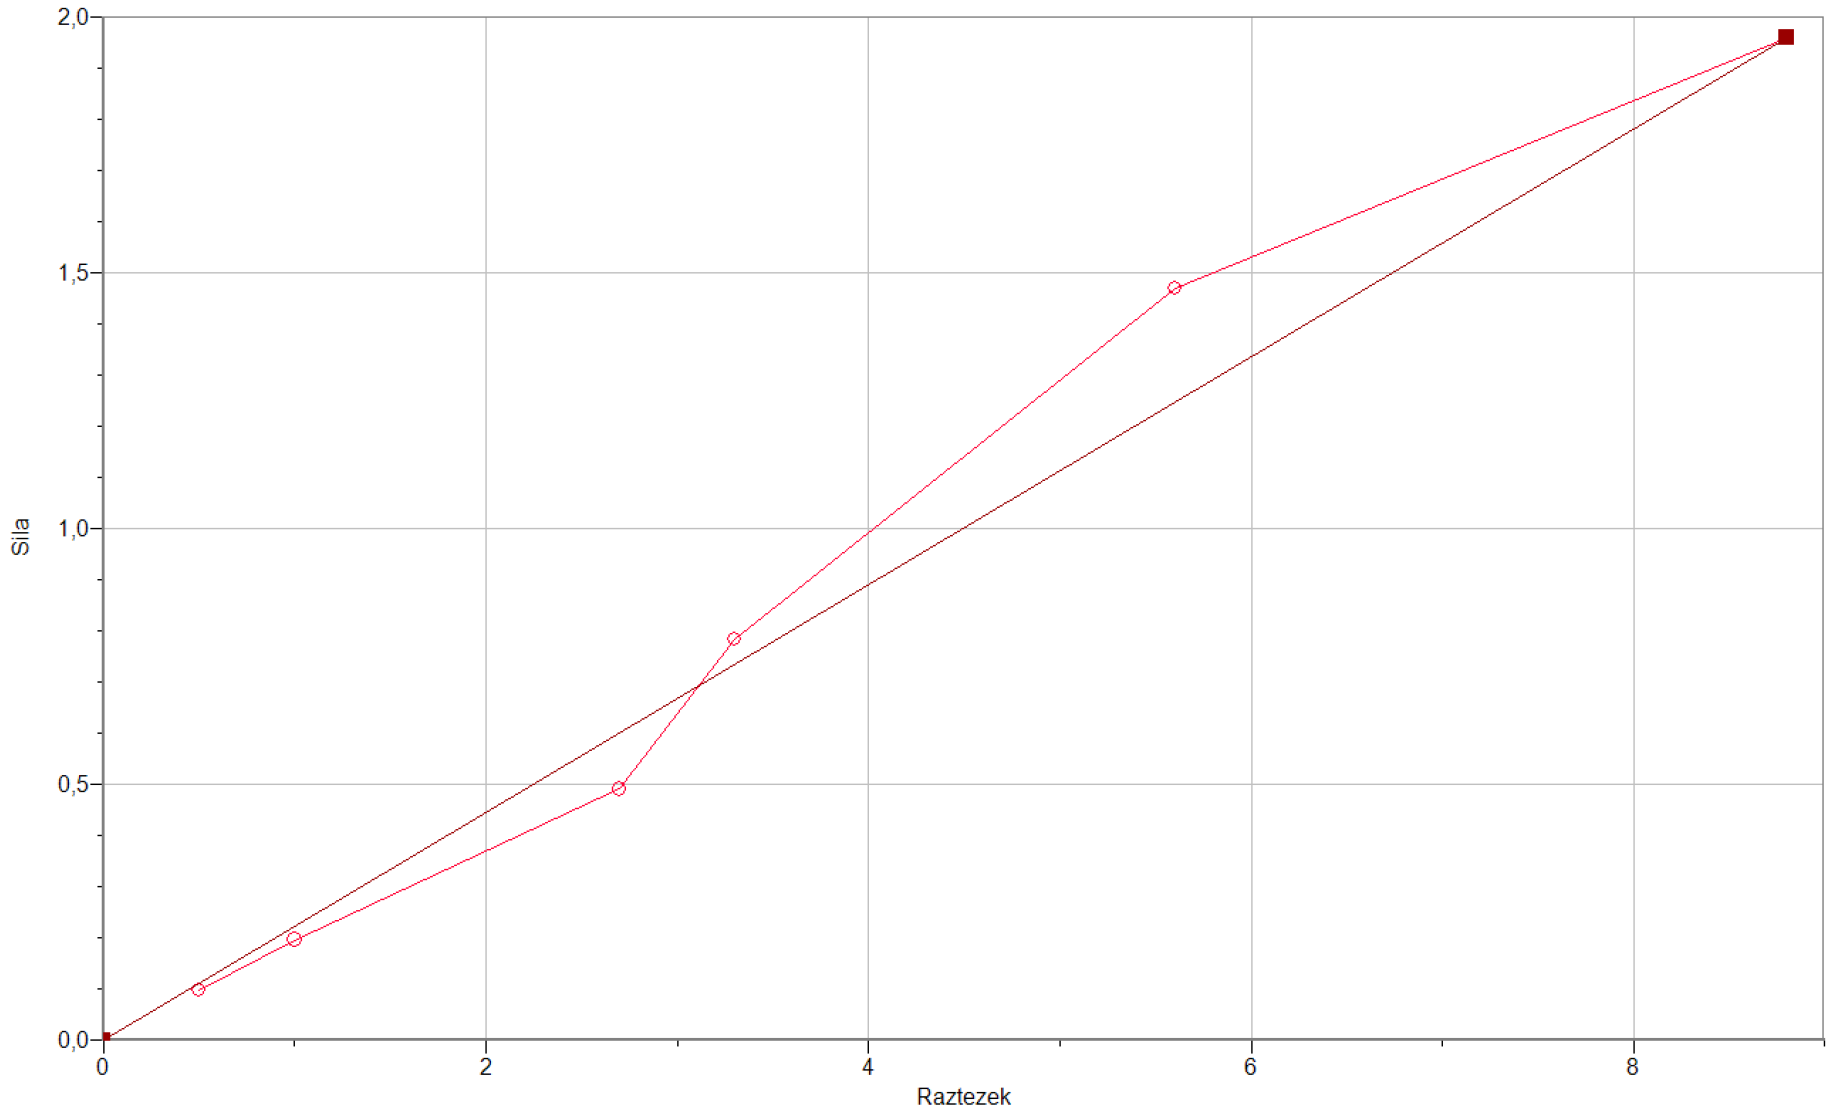
\includegraphics[width=\textwidth]{KoeficientK}

Koeficient k:

\[
  k = \frac{F_2 - F_1}{\Delta x_2 - \Delta x_1} = 40Nm (1 \pm 0,02)
\]

Razdalja od prijemališča vzmeti do osi $d = 18 cm (1 \pm 0,1)$

Koeficient navora D' se izračuna po enačbi:

\[
  D' = kd^2 = 1,3 Nm (1 \pm 0,03)
\]

\section*{Izračunani $t_0$, $ t_1$, $ t'$, $ T$, $\omega_0$, $\omega_1$, $\omega'$ in $ \omega_u$}

\begin{center}
  \begin{tabular}{| c | c | c | c | c |}
    \hline
    & $t_0$ & $t_1$ & $t'$ & $T$ \\ \hline
    izmerjeno & 1,85s & 1,70s & 1,85s & 16,64s \\ \hline
    izračunano & 1,85s & 1,76s & 1,80s & 36,20s \\ 
    \hline
  \end{tabular}
\end{center}

\begin{center}
  \begin{tabular}{| c | c | c | c | c |}
    \hline
    &  $\omega_0$ & $\omega_1$ & $\omega'$ & $\omega_u$ \\ \hline
    izmerjeno & $3,40s^{-1}$ & $3,71s^{-1}$ & $3,40s^{-1}$ & $0,38s^{-1}$ \\ \hline
    izračunano & $3,39s^{-1}$ & $3,78s^{-1}$ & $3,59s^{-1}$ & $0,39s^{-1}$ \\
    \hline
  \end{tabular}
\end{center}

Razen čas utripanja, se podatki razlikujejo zgolj na stotinke. Zakaj se čas utripanja tako razlikuje, je napisano pod delom Čas utripanja - izračunano

\section*{Faktor sklopitve}

Faktor sklopitve se izračuna po formuli:

\[ 
  K = \frac{D'}{D+D'} = \frac{1-(\frac{\omega_0}{\omega_1})^2}{1 + (\frac{\omega_0}{\omega_1})^2}
\]

\subsection*{Izmerjeni podatki}

\[
  K =  0,09 (1 \pm 0,1)
\]

\subsection*{Izračunani podatki}

\[
  K = \frac{D'}{D+D'} = 0,1(1 \pm 0,2)
\]


                                                                                                                                                                         
\end{document}
